\begin{frame}
\frametitle{Fraction of Recombinant Chromosomes (FRC)}
 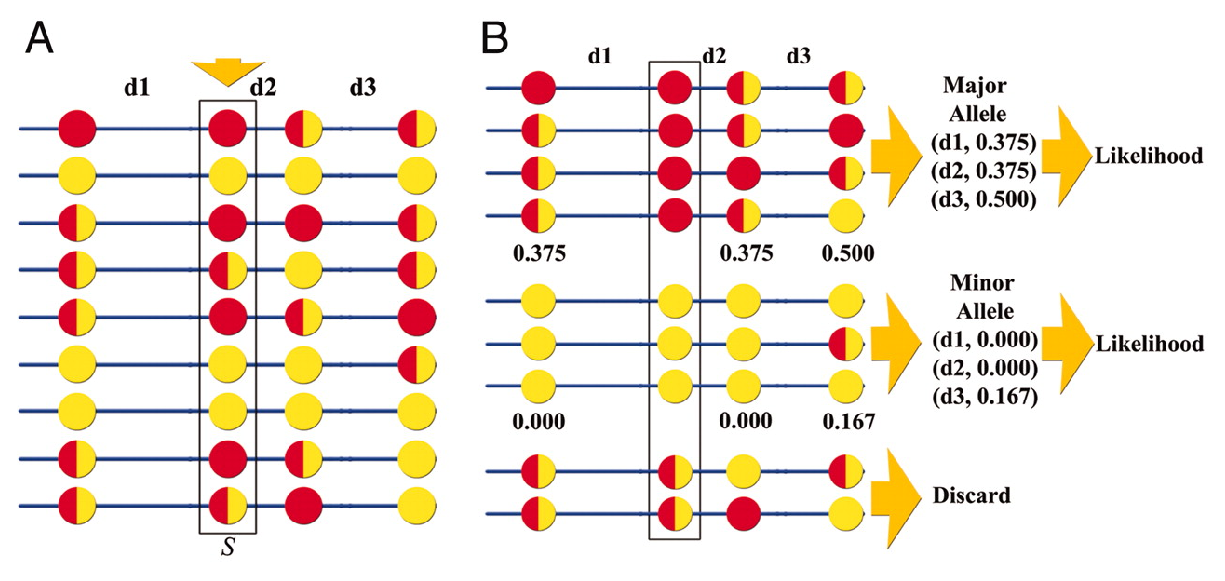
\includegraphics[width=\textwidth]{wang-frc.eps}
\end{frame}

\begin{frame}
\frametitle{Relating FRC to gamete frequencies}
\psset{unit=2cm}
\centering
\begin{pspicture}(4.5,2.4)
\rput[b](1.1,2.2){\large $A$-gametes}
\rput[b](3.5,2.1){\large $a$-gametes}
\pscircle(1.1,1.1){1.1}
\pswedge*[linecolor=blue](1.1,1.1){1.1}{200}{340}
\rput*(1.1,0.4){$AB$}
\rput*(1.1,1.4){$Ab$}
%
\pscircle(3.5,1.1){1}
\pswedge*[linecolor=blue](3.5,1.1){1}{170}{10}
\rput*(3.5,0.7){\large $aB$}
\rput*(3.5,1.6){\large $ab$}
\end{pspicture} Calculated for $A$ and $a$ separately.  
\pause For $A$-gametes, FRC approximates the frequency of $AB$ (the rare
type) among $A$-gametes.  \pause For $a$-gametes, FRC approximates the
frequency of $ab$ (the rare type) among $a$-gametes.
\end{frame}


%\begin{frame}
%\frametitle{FRC in terms of haplotype frequencies}
%\begin{center}
%\begin{tabular}{lcccc}
%Haplotype & AB & Ab & aB & ab\\
%Frequency & $x_1$ & $x_2$ & $x_3$& $x_4$\\
%\end{tabular}
%\end{center}
%\begin{eqnarray*}
% \hbox{FRC} &=&  p_{b|A} / p_{B|a}\\
%            &=& \underbrace{\left(\frac{x_2}{x_1+x_2}\right)}_{p_{b|A}} 
%                \Bigg / 
%              \underbrace{\left(\frac{x_3}{x_3+x_4}\right)}_{p_{B|a}} 
%\end{eqnarray*}
%\end{frame}

\begin{frame}
\frametitle{At a given site}
\begin{itemize}
\item FRC increases with time.  
\pause
\item Rate of increase depends on recombination rate.
\end{itemize}
\end{frame}

\begin{frame}
\frametitle{At a given time}
\begin{itemize}
\item FRC increases with distance along the chromosome.
\pause
\item Rate of increase is fast near neutral sites.
\begin{quote}
(Neutral $\Rightarrow$ old $\Rightarrow$ lots of recombination.)
\end{quote}
\pause
\item Rate is slow near ongoing selective sweeps.
\begin{quote}
(Selected $\Rightarrow$ young $\Rightarrow$ little recombination.)
\end{quote}
\end{itemize}
\begin{block}{Recipe}<4->
Look for regions where FRC is low in big sections of
chromosome. 
\end{block}
\end{frame}
